\documentclass[11pt,a4paper]{article}
\usepackage[english]{babel}
\usepackage[utf8]{inputenc}
\usepackage[babel, style=english]{csquotes}

\usepackage[T1]{fontenc}
\usepackage{graphicx}
\usepackage{amsmath}
\usepackage{amsthm}
\usepackage{amssymb}
\usepackage{wrapfig}
%\usepackage{algorithm}
%\usepackage{algpseudocode}
\usepackage{tikz}
\usepackage[export]{adjustbox}
%\usepackage{cite}
\usepackage{url}
\usepackage{tocloft}

\usepackage{todonotes}
\usepackage{xcolor} % Required for specifying custom colors
\usepackage{caption}
\usepackage{regexpatch}


\parindent 0pt
\parskip 12pt

\graphicspath{ {figures/} }

\title{Convoluational Neural Networks for German Roadsign Detection}
\author{Roman Schulte-Sasse}
\date{\today}

\begin{document}
\maketitle
\clearpage


\section{Introduction}
Extracting the contents of a digital image has been proven to be a hard problem for computers. Since for them, an image is only a matrix of values, knowing what structures a human would recognize in this image, is a non-trivial problem.\\
Yet it is a problem crucial to solve for a wide range of modern problems. In autonomous driving, for instance, an autonomous car has to manage to drive in a system designed for humans.\\
Since the environment of a street is highly dynamic and subject to often unpredictable changes, the car must not solely rely on its GPS sensors in combination with maps to know the current speed limits or similar.

Simply put, for a autonomous car to be able to react to such rapid changes in the environment (eg. road works, accidents, etc), it must acquire information from road signs.
Such a problem can be interpreted as a classical machine learning problem on images, in which a computer has to determine to which class an image belongs.
The german road sign recognition challenge (GRSRC) tries to solve that problem by supplying a training dataset from which a computer can learn the structure of images belonging to each of the classes.

Deep neural networks have become the state-of-the-art solution to extract meaning from computer images or videos \cite{lecunConvADF}. They have been proven to achieve maximum accuracy when trying to classify such material into different classes. However, as many techniques in machine learning, classical aNNs have a very large number of parameters when the input is high dimensional. This high number of parameters which have to be tuned during training, renders aNNs infeasible when the image is directly taken as input for a neural network.\\
While there have been approaches to detect features in images and let the neural network learn on them, these preprocessing steps most often introduce a bias to the model which is generally not wanted \cite{shamir2010pattern}.\\
Convolutional architectures overcome the \textit{curse of dimensionality} by reducing the number of parameters to tune drastically. Furthermore, they exploit properties that are always present in images and render the learning algorithm translation invariant.\\
For these reasons, I chose to train a convolutional neural network on the GRSRC data set. In the challenge, there were different groups participating that used a similar approach and my architecture and preprocessing was heavily influenced by the work of Sermanet et al. \cite{sermanet2011traffic}

I will firstly present the neural network training algorithm and it's convolutional counterpart. From there, I will show how the data set was preprocessing and how this resulted in better classification. Finally, I will evaluate the work and show how the trained network may aide in the automatic classification of German roadsigns only using a camera mounted in the vehicle.

\section{Neural Networks \& Convolutional Neural Networks}
Artificial neural networks have become the state-of-the-art machine learning system for applications in computer vision, natural language processing and robotics.\cite{visionANN, nlpANN, roboticsANN} They can be seen as an ensemble of different linear classifiers that are put together to solve a non-linear problem. While each of the individual classifiers only solves a linear sub-problem, the network is able to solve highly complex classification and regression tasks.\\
In a more formal way, we can define a fully connected feed forward neural network as a directed and acyclic graph in which the nodes are arranged in layers. Nodes within one layer have no connections to each other but every node from layer $i$ is connected to all nodes in layer $i+1$ and $i-1$.\\
The connections between nodes have weights associated with them. Nodes can also be called neurons, or units.
\begin{figure}[h!]
	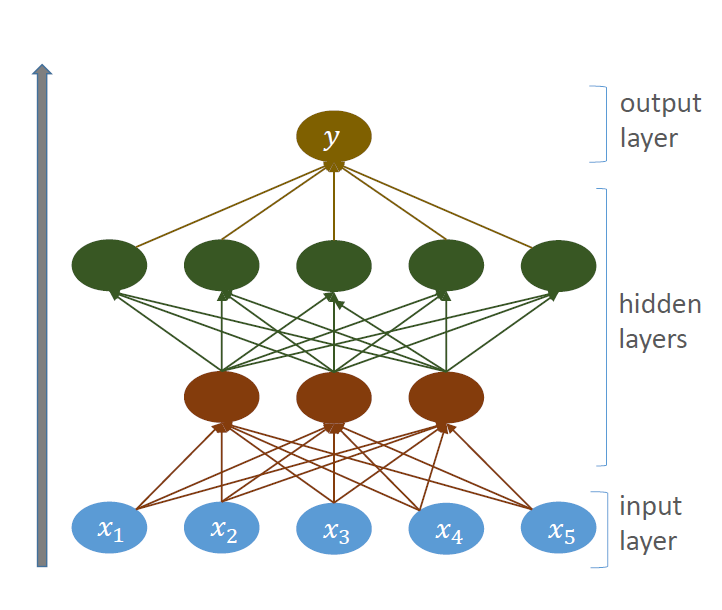
\includegraphics[width=0.8\textwidth]{ann_forward.png}
	\centering
	\label{fig:ann}
	\caption[Artificial Neural Network]{A schematic view of a fully connected feed forward network. The 5-dimensional input vector is first forced to be represented by only three dimensions (red layer). This reduced representation is then seen by the next layer (green layer) which tries yet again to find another representation of the input data.Finally, a one-dimensional output classifies the input vector.}
\end{figure}
To classify a data vector, it is clamped to the lowest layer of the network and then propagated upwards. This way, each neuron can be viewed as a linear classifier that takes a certain responsibility in the search space. In image recognition, a neuron might be responsible for detecting horizontal edges in an image, while a neuron further up the network might be responsible for deciding whether there is a cat in the image or not.\\
Feed forward neural networks are a supervised method, which means they need labels for input vectors in order to learn from the data. When a new training vector is shown to the network, the information is first propagated up and compared to the expected output. From there, an error is calculated and its derivative with respect to the weights connecting units makes the network minimize the classification error.\\
Calculating the partial derivative of the error function with respect to one of the weights is an iterative process. First, the derivatives for the deepest layer are calculated and from there it becomes possible to calculate them for the second-deepest one and so one. This top-down approach is why the algorithm is called backpropagation, because it starts at the back and propagates the partial derivatives back to the front.

\subsection{Training Neural Networks}
The backpropagation algorithm tries to answer the question, in how far each of the neurons are responsible for the error that was made by the network as a whole. That means, when we propagate the error up to the output layer, we then first calculate the output's error, using the \textit{squared error} measure.
\begin{equation*}
E = \frac{1}{2} \sum_{i=1}^k (y_i - t_i)^2
\end{equation*}
This error is then split up between all neurons in a top-down fashion. The key principle is here to calculate the error's partial derivatives with respect to the weights that connect that two neurons. We start by calculating the derivative for the weights connecting the output layer with the second-last layer. These can be calculated easily with the \textit{chain rule}. From that point, it becomes possible to calculate the derivatives for the weights connecting the second-last with the third-last layer and so on. Finally, we arrive at the input layer and the backpropagation algorithm terminates for the given input. When we repeat this procedure for all data points, the network will slowly start to learn to minimize the error.\\
Traditionally, neural networks were trained using the \textit{sigmoid activation function} which is given by:
\begin{equation*}
sig(x) = \frac{1}{1 + e^{-x}}
\end{equation*}
This function is particularly handy because of its very easy derivative. We can write:
\begin{equation*}
sig'(x) = sig(x) (1-sig(x))
\end{equation*}
So the question that asks in how far one unit is responsible for the error of the whole network becomes a question of partial derivatives with respect to the connections between layers (the weights). The \textit{chain rule} states how the derivative for functions that were applied one after the other can be written, using only the single functions. More precisely, the chain rule states:
\begin{equation} \label{eq:chainrule}
(f \circ g)' = (f' \circ g) \cdot g'
\end{equation}
When we consider the neurons as functions that are applied one after the other, we can finally calculate the partial derivatives.\\
During the forward step, the output and input of each neuron is stored. Let $o_i^k$ be the output of neuron $i$ in layer $k$ and $h_j^{k+1}$ be the input for neuron $j$ in layer $(k+1)$. These values are known from the forward pass and can be used to calculate the partial derivative with respect to the weights.
\begin{equation*}
\frac{\partial E}{\partial w_{ij}^k} = o_i^k \delta_j^{(k+1)}
\end{equation*}
where $\delta_j^k$ is given by:
\begin{equation*}
\delta_j^k = \begin{cases}
	f'(h_j^k) (t_j - o_j^k), & \text{for output layer}.\\
	f'(h_j^k)(\sum_{i \in incoming} w_{ji} \delta_i^{(k+1)}, & \text{for inner layers}.
\end{cases}
\end{equation*}
\begin{figure}[h]
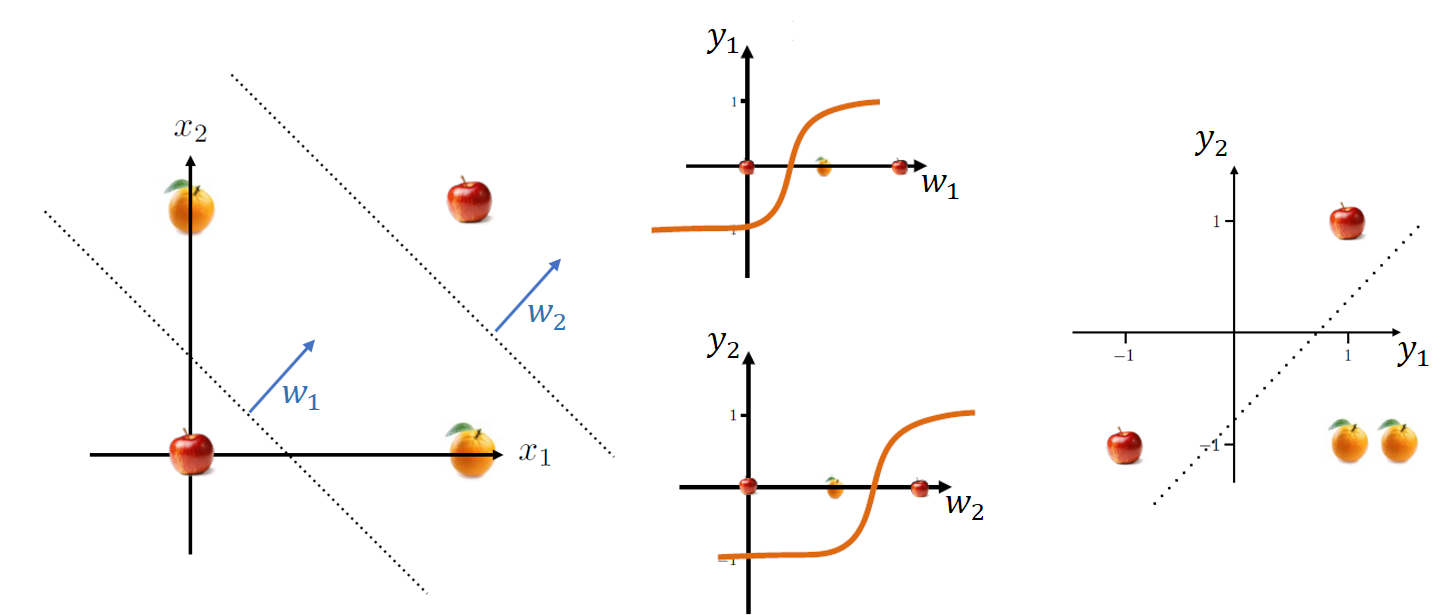
\includegraphics[width=0.9\textwidth]{ann_intuition.png}
\centering
\caption[Hierarchical Learning in aNNs]{Example of how a neural network can solve the XOR problem. The first layer of the network only finds good data representations that serve as input for the next layer. There, the problem is suddenly linearly separable, and the problem as a whole can be solved.}
\label{fig:annIntuition}
\end{figure}
The backpropagation algorithm has the tendency to find useful representations of the data in the first layers, as is depicted in figure \ref{fig:annIntuition}. This property yields in a high interpretability of neural networks despite their complexity.

However, neural networks have also some disadvantages. Because of the large amounts of parameters, the classical fully connected feed forward network requires huge amounts of training data for successful learning. Overfitting can occur easily and does so frequently. Furthermore, there is no guarantee that the solution found by the network is optimal in any way.

Also, neural networks have suffered from the \textit{vanishing gradient problem}. This problem comes from the nature of the sigmoid activation function which "squeezes" the output of any layer to be between zero and one. Respectively, the backpropagation algorithm only updates the parameters in the upper layers because the whole error "is used up" by those, while leaving the most important first layers untouched \cite{hochreiter1991}.
\begin{wrapfigure}[14]{r}{0.52\textwidth}
	\vspace{-1pt}
	\begin{center}
		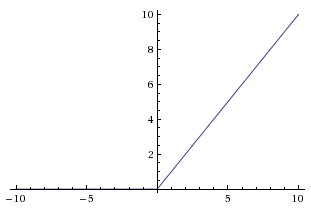
\includegraphics[width=0.5\textwidth]{relu.jpeg}
	\end{center}
	\vspace{-1pt}
	\caption{The rectified linear activation function}
	\vspace{-1pt}
	\label{fig:relu}
\end{wrapfigure}
Recent advances in the field promoted the \textit{rectified linear unit} (ReLU) as activation function of choice in most applications \cite{hahnloser2000digital}. This function is given by:
\begin{equation*}
f(x) = max(0, x).
\end{equation*}
The ReLU activation assigns large derivatives when the error is large and thus gets rid of the vanishing gradient problem.

Finally, an additional drawback of traditional feed-forward neural networks lies in the application to images. Because of the large number of dimensions when applied directly on the pixels (one dimension per pixel), it is usually not feasible to train neural networks on large images without running in the above problem of overfitting.\\
And also, neural networks are not translation invariant. That is, when there is the same pattern of pixels somewhere in the image, we usually want it to be recognized as such, no matter where the pattern is located in the image. But imagine a neural network that is trained to see some feature (an apple, for instance) in the upper left corner. The network would be unable to recognize the very same apple located in the lower right corner of the image when this image was not part of the training set.

To overcome these problems, LeCun et al. proposed the convolutional neural network in \cite{cnnOriginal}, which resolves most of the problems in the field of computer vision applications.

\subsection{Convolutional Neural Networks}
The convolutional neural network is a variant of the conventional neural network in which the connections between two units are convolutions instead of simple connections. The convolution operation is very complex and has different applications in different scientific fields but it is worth noting that convolutions can be regarded as filters or kernels applied to images.\\
With this informal definition, we can define the weights connecting the input layer with the first one as filters. Their application to the image (the input layer) yields in the first hidden layer of the network. When we have a two-dimensional image of $x \times y$ input neurons, the first hidden layer typically is three-dimensional. This is because we apply many filters to the image, each one of them producing a two-dimensional matrix.\\
When we now look at the mathematical side of it, we only have to change the way gradients are computed from the error. Since the connection between layers is a convolution, we can also express the gradient as convolutions.

This approach solves the translation invariance issue because a filter will be applied everywhere in the image. Furthermore, the number of parameters is drastically reduced. When we use $k$ different kernels, each of size $x_k \times y_k$, we have $k \cdot (x_k \cdot y_k)$ parameters for the convolutional layer. Typically, $x_k$ and $y_k$ are small and 20-30 kernels are often enough to describe the structure of an image.\\
\begin{figure}[h]
	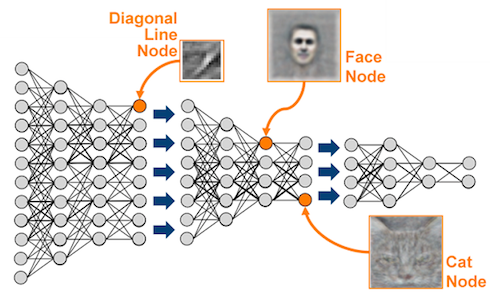
\includegraphics[width=0.8\textwidth]{deep-learning.png}
	\centering
	\caption[Deep Convolutional Neural Network]{Schematic view of a deep convolutional neural network. The first layers capture low-level features like edge-detectors in the images. Later stages of the network capture more complex features like cats or faces. Source: \cite{deepNetworkImage}}
	\label{fig:deeplearning}
\end{figure}
For applications in image recognition or computer vision, the interpretability is increased when using convolutional neural networks because the kernels have an interpretation that is known already. The kernels usually correspond to stereotypical mini-images like the cat or the face in figure \ref{fig:deeplearning}.

\section{German Road Sign Detection}
Training a convolutional neural network means to present to it all the images in a database for which the labels are known. In our case, there are 43 different classes of road signs with the images being of different sizes and scales. The road sign in an image can be anywhere in the image and partly covered. There are 39252 images in total provided by the GTSRB (German Traffic Sign Recognition Benchmark).\\
Because the parameters are optimized by gradient descent, it is often a good idea to present all of the training data multiple times until training has converged to a (local) minimum. Furthermore, the network requires all images to have the same dimensions which is not the default in the GTSRB data set.\\
Also, it is often recommended to artificially increase the number of training examples by adding rotated and scaled versions of the images.

\subsection{Preprocessing}
In order to make the provided images useable for a cNN, I had to transform them to be of the same dimensions. I decided to scale all images to a square size of $32 \times 32$ pixels. The smallest images in the data set are as little as $15 \times 15$ pixels while the largest were of size $250 \times 250$.\\
As a next step, I did a normalization over the luminosity of the images. Since some of the training examples are very dark or over-exposed, this step is crucial to achieving high performance.\\
After the normalization step, all channels but the Y-channel (of a YUV image) were removed, resulting in a set of gray-scale images.\\
Afterwards, the data set was \textit{blown up} by adding randomly transformed copies of randomly selected images to it. First, I split the data set into training and test sets. The data sets contain around 35000 examples for training and 4000 for testing (with a ratio of $~9\%$ testing images). By inflating the data with artificially transformed images, the final data set contained 100,000 training examples while the test set was not modified.\\
From the resulting training and test set, a matrix representation was derived and stored to make generic loading of differently preprocessed data sets possible. The preprocessing step is also memory intensive so that it might be better to perform these calculations on a different server than training.

\subsection{Training \& Network Parameters}
The data as described above can now be used for training a deep convolutional neural network. As shown by LeCun et al. in \cite{cnnOriginal}, two convolution stages are often more expressive than just a single one as the second convolutional layer learns more sophisticated features from the data. This is due to the fact that the second layer only sees the data represented by the first layer.\\
For training, I used the \textit{tensorflow} framework \cite{abadi2015tensorflow} which allows to formulate a computational graph which is then heavily optimized by the internal tensorflow compiler. Furthermore, the framework allows for execution of most of the instructions in a computational graph on GPUs. Graphics processing units are known to accelerate computations by massively parallelizing them and especially with convolutions, they can be much faster than their CPU optimized equivalents \cite{cudnn}. Another advantage of tensorflow and similar frameworks, such as \textit{theano}, \textit{torch} or \textit{keras} is the automated computation of derivatives. In such a framework, the parameters can be adapted using one of many different optimizers. I chose the \textit{adam} optimizer \cite{overviewGD} as it is one of the most effective gradient descent optimizers that includes many different ideas, such as \textit{momentum}, \textit{nesterov} and many more.
\begin{figure}[h!]
	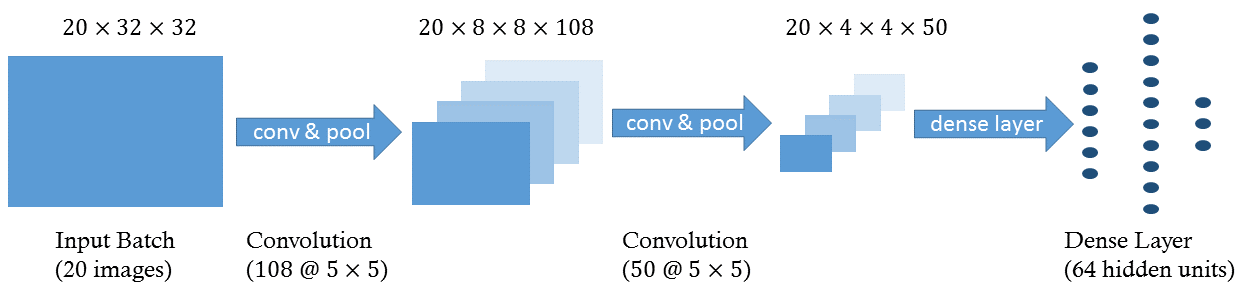
\includegraphics[width=\textwidth]{cnn_architecture.png}
	\centering
	\caption[Architecture]{Architecture of the cNN to learn german road signs. The network contains of two convolution layers that are max-pooled afterwards. The resulting shrinked layer is then flattened and densely connected to the output layer. This layer also uses \textit{dropout} to improve the robustness of predictions.}
	\label{fig:architecture}
\end{figure}

There are many \textit{hyper parameters} to cNNs, such as the learning rate or kernel sizes to use. With most parameters, I closely sticked with the paper of Sermanet et al. \cite{sermanet2011traffic} but with some not.\\
The learning rate I used is much smaller than in the paper which might be related to the choice of optimization algorithm. The adam optimizer should adapt the learning rate in a procedure similar to \textit{r-prop} but a very small learning rate in the beginning can be crucial to get some good first feature detectors. Because of the computational complexity, I decided not to search automatically for good hyper parameters as suggested by \cite{gridsearchHyperparams}. The batch size was also modified since there is simply not enough memory on the graphics card used to process more than around 20 images in one batch. Larger batch sizes usually result in more robust learning while \textit{online learning} (batch size of one) makes the gradient descent somewhat "jumpy".\\
Kernel sizes were adapted from \cite{cnnOriginal} to a size of $5 \times 5$ which is the de-facto standard kernel size for image classification. After each convolution layer the result is max pooled to reduce the size of the layer. Pooling adds some small translation invariance to the algorithm but mainly results in a pyramidal structure of the network. That effects makes sure that layers further up learn much more high-level representations of the data than the lower layers (cf. figure \ref{fig:deeplearning}).

After convolutions took place, the remaining small images ($4 \times 4$) are flattened and transformed by a \textit{ReLu} layer. Each neuron in the hidden layer of that sub-network is connected to each pixel of the last convolution stage. It receives a weighted sum of all of these pixels as input and transforms that using the non-linear \textit{rectified linear activation function}. In my network, there are 64 hidden ReLu units.
The dense layer is then connected to the output layer which consists of 43 units. The result is encoded as one-hot-representation, meaning that each output unit represents one of the 43 classes. The classification result is obtained by using the argmax function over the 43 classes, thus choosing the class for which the network assigns the highest probability.\\
The labels are equivalently also encoded as a 43-dimensional vector with only zeros except for the class to which the training image belongs.

\section{Evaluation \& Outlook}
The convolutional neural network achieves an overall accuracy of $~99 \%$ on the test set. That data was never shown to the network and was subtracted from it before blowing up the training set.\\
\begin{figure}[h!]
	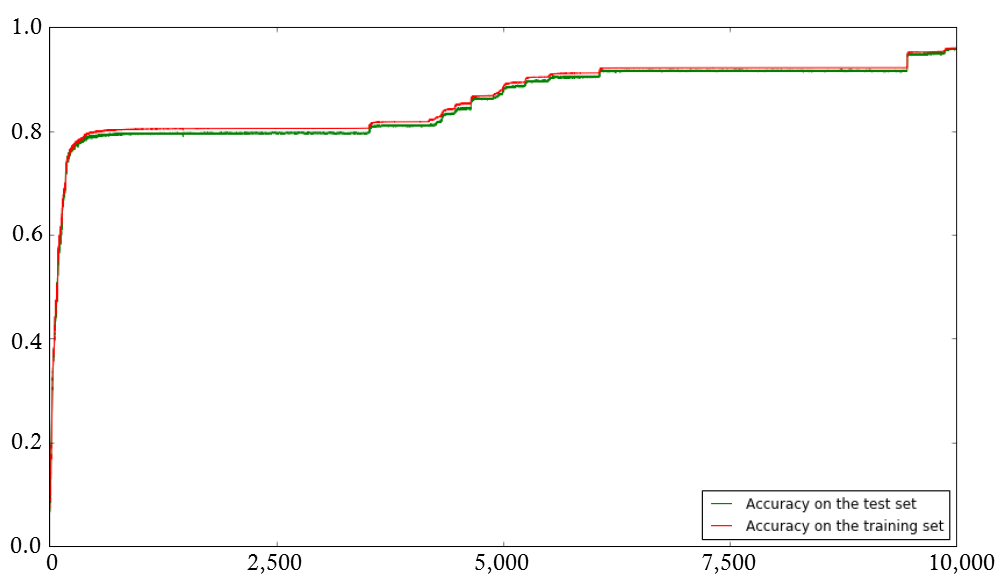
\includegraphics[width=\textwidth]{accuracy.png}
	\centering
	\caption[Accuracy]{The accuracy over training and test set. On the x-axis, the number of epochs is shown while the y-axis depicts the accuracy on training and test set. From the training set, there was a random subsample chosen to reduce computations. As expected, the test error is a little higher than the training error but the two do not diverge.
}
	\label{fig:accuracy}
\end{figure}
From the plot in figure \ref{fig:accuracy} we can clearly see that the training is successful. Not only does the accuracy start at random in the first epoch (which would be $\frac{1}{43} = 2 \%$) but it increases rapidly in the beginning and stagnates afterwards. From there, the training does not change much for a long time until suddenly there is again an increase in the accuracy. One possible explanation for that behavior might be a local minimum of which the gradient descent algorithm can only escape through a random configuration or a long "ridge" in which the gradient is almost zero but not quite.\\
However, the classification accuracy increases during training and we cannot yet observe overfitting. That indicates that a longer training would be promising as there can still be improvements until the time when overfitting occurs in the model.

The overall accuracy is the measure of how well the algorithm classifies images into their respective class but it does not measure the ratio of true positives to false positives. This is exactly what a \textit{receiver operator characteristics} (ROC) curve tells us and the measure is much more precise when dealing with unbalanced training and test sets.
\begin{figure}[h!]
	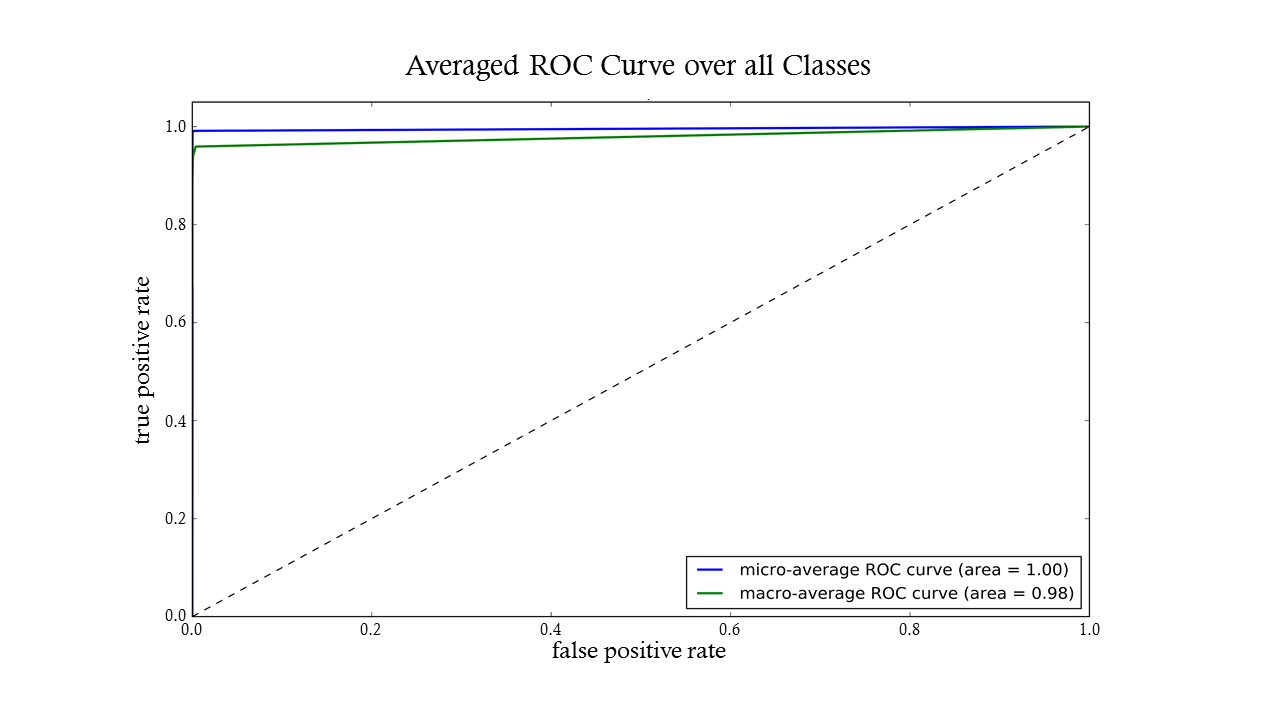
\includegraphics[width=\textwidth]{roc_multi.png}
	\centering
	\caption[Average ROC Curve]{ROC curve for a multiclass settings. The two curves represent two interpolated versions of a mean ROC curve over all classes.}
	\label{fig:roc_avg}
\end{figure}

In figure \ref{fig:roc_avg} we see an interpolated ROC curve over all classes. A ROC curve measures the true positive rate against the false positive rate and can provide information on how many errors one has to tolerate in order to have a desired specificity. With a perfect classification, the curve would be in the upper left corner.\\
In our case, however, we can conclude that we can get around 90-95 \% true positives without any false positives over all classes.
\begin{figure}[h!]
	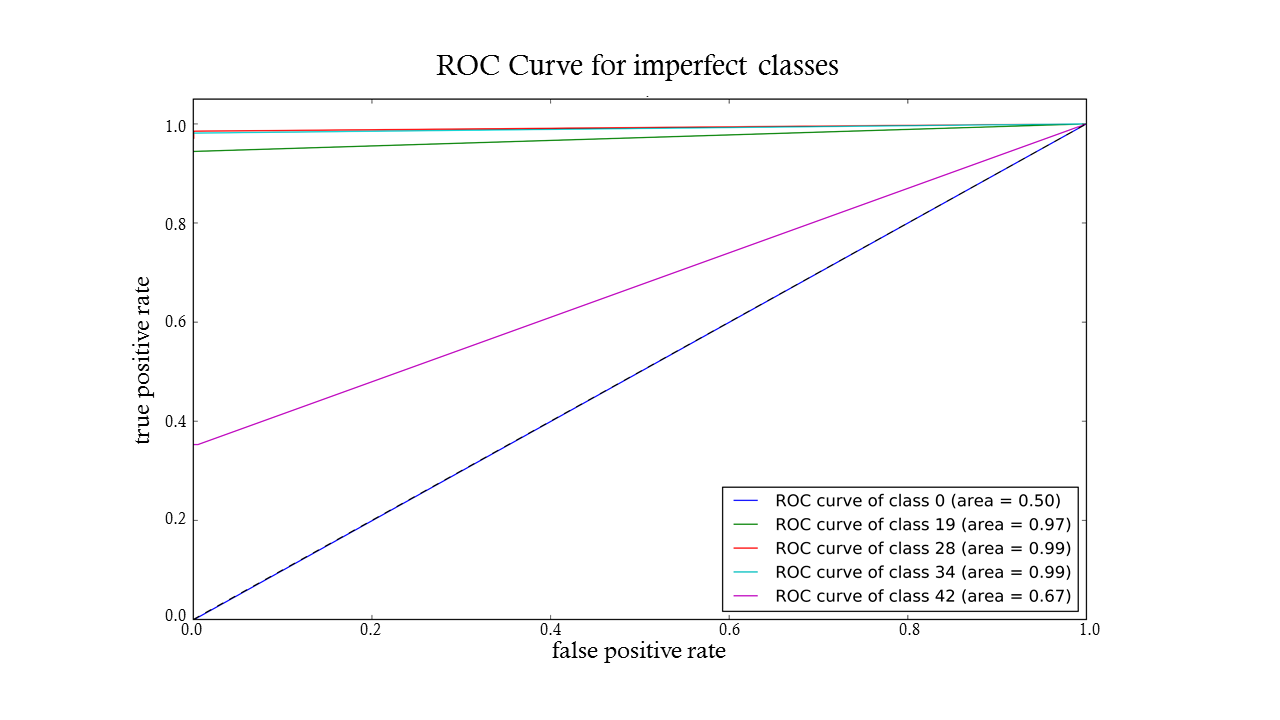
\includegraphics[width=\textwidth]{roc_imperfect.png}
	\centering
	\caption[ROC Curve for imperfect classes]{ROC curve showing only those classes that did not achieve perfect classification on the test set. While most of these classes range between $97 - 99 \%$ there are four classes that the algorithm is not able to classify at all and one class where it is merely better than random (with an AUC value of $68\%$).}
	\label{fig:roc_imp}
\end{figure}

On the other hand, when we look at the specific classes this changes a lot. As figure \ref{fig:roc_imp} suggests, there seems to be many classes that the algorithm can classify almost perfectly while it has problem with a few of the road signs. In these rare cases, the network only achieves random classification.\\
It is not yet clear why this might be the case but future versions of the cnn should pay attention to these classes as they are indicated here to be hardest to classify.

While the convolutional neural network presented in this paper is clearly able to generally classify german road signs very well, there is still much work to be done. First of all, the camera of an autonomous car only extracts whole images from which the area in which a road sign might be positioned has to be extracted. This can be done using the depth sensors or colors for finding possible candidates. Furthermore, we only looked at images that do contain road signs. In order to make the application practical in the real world, the algorithm should be able to reject all images that do not contain any road sign, such that the extraction algorithm may have a high false positive rate.\\
And finally, autonomous driving is a very dangerous field. While classification results of 95\% is very high, much attention should be paid to what happens when road signs are falsely identified. Human classification for the data set at hand was around 98.8\%, but in a typical driving situation there are many images from which the camera can extract the correct road sign. So careful modeling of the detected road signs is a vital part for an autonomous car to drive safely.
\newpage
\bibliography{bibliography}
\bibliographystyle{plain}

\end{document}